\documentclass[UTF8]{ctexart}

\usepackage{subfiles}  

%下面的语句, 引入你的头部设置文件
\usepackage{C:/phpStorm_proj/02_myself_ID_EGO/+100_latex_all_math_sel/myPreamble} 
%必须是绝对路径,才能让各个tex在单独编译时使用到

\title{文件名}


%---------------------------------


\begin{document}
	\tableofcontents % 生成目录
	\date{} % 若不写这句, 则默认也会渲染出日期, 所以我们要手动赋空值
	\maketitle  %这行代码, 让你前面的 title, author, date生效
	
	
	
	\section{离散型 : 超几何分布 : \\ $\boxed{
			P\left\{ X=k\text{女} \right\} =\frac{C_{\text{女总数}}^{\text{取}k}C_{\text{男总数}}^{\text{取}n-k\text{人}}}{C_{\text{总}}^{\text{取}n\text{人}}},\ \ k=0,1,...,\min \left\{ n\text{人,女总数} \right\} 
			}$}
	
	超几何分布  (Hypergeometric Distribution), 是统计学上一种离散概率分布. 它描述了: 从有限的N个物件(其中包含M个``指定种类的物件") 中抽出n个物件(不放回). 这n个物件中, 含有k个``指定种类的物件"的概率. \\	
	
	\textbf{简单记忆就是: 从总数N个人中(其中包括了总数M个女人, 则男人数量就是 N-M), 抽出n人, 能取到k个女人的概率.} \\
	
	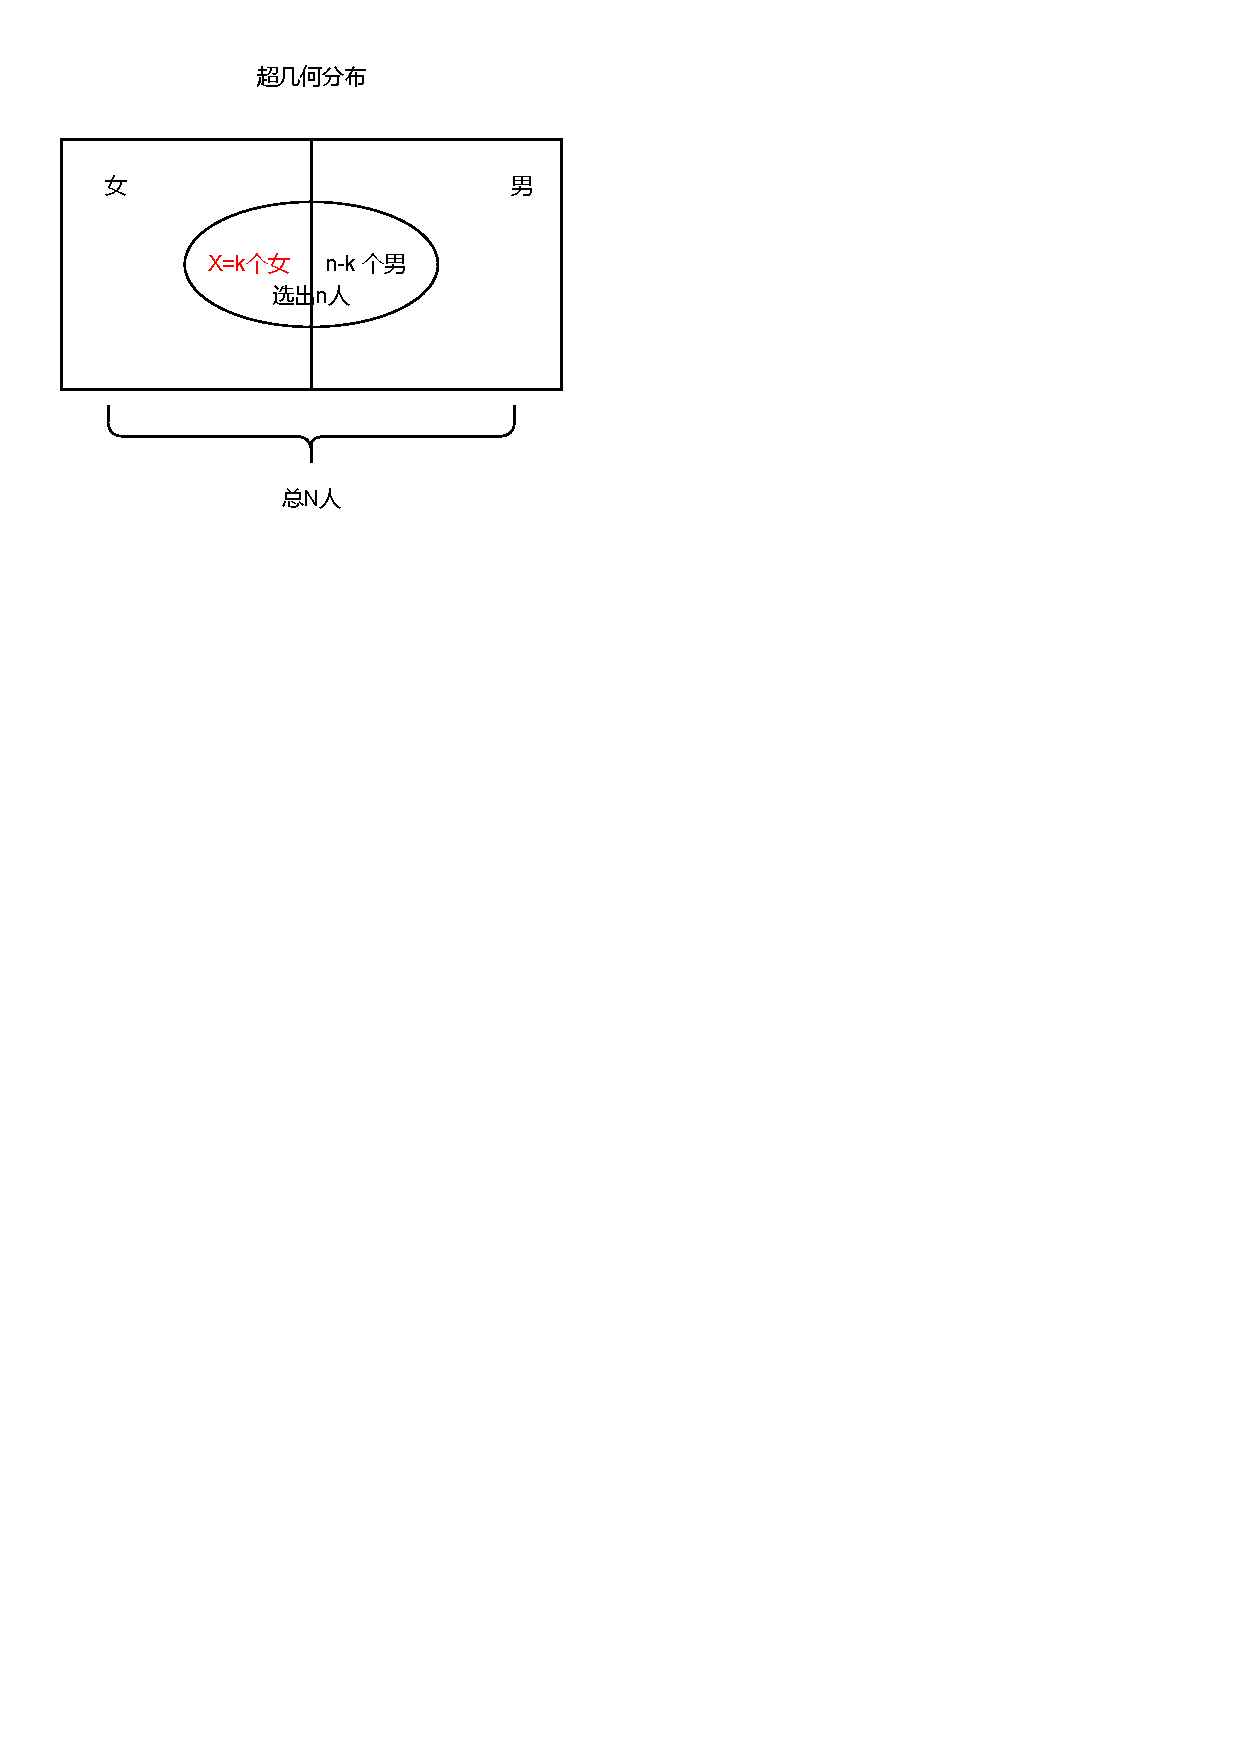
\includegraphics[width=0.5\textwidth]{/0162.pdf} \\
	
	$\boxed{
	P\left\{ X=k\text{女} \right\} =\frac{C_{\text{女人总数}}^{\text{取}k\text{人}}C_{\text{男人总数}}^{\text{取}n-k\text{人}}}{C_{\text{总人数}}^{\text{取}n\text{人}}},\ \ k=0,1,...,\underset{\text{取两者中最小的那个}}{\underbrace{\min \left\{ n\text{人,女人总数} \right\} }}
	}$ \\
	\vspace{1em} 
	
	\begin{myEnvSample}
		有共20人, 其中5女, 15男. 任取4人. 即,  \\
		- X : 表示所抽取的4人中, 女生的人数. 
						
		\begin{align*}  % 支持每行编号. 若不需要编号, 就用 align*环境
	&P\left\{ X=k\text{女} \right\} =\frac{C_{\text{女总}}^{\text{取}k}C_{\text{男数}}^{\text{取}n-k\text{人}}}{C_{\text{总}}^{\text{取}n\text{人}}},\ \ k=0,1,...,\min \left\{ n\text{人,女人总数} \right\}\\
&P\left\{ X=k\text{女} \right\} =\frac{C_{5\text{女}}^{k\text{女}}\cdot C_{15\text{男}}^{4-k\text{女}}}{C_{20}^{4}},\ k=0,1,...,4
		\end{align*}
	
	比如, 所取的4人中, 有2女的概率是 : \\
	$	P\left\{ X=k=2 \right\} =\dfrac{C_{5}^{2}\cdot C_{15}^{4-2}}{C_{20}^{4}}=0.216718	$ \\
	
	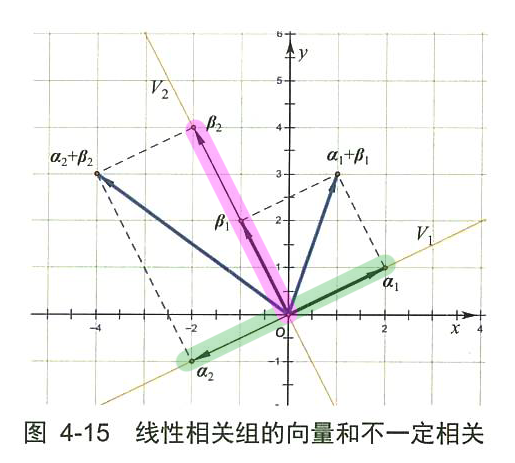
\includegraphics[width=0.9\textwidth]{/0162.png}	
	\end{myEnvSample}
	
	
	
	
\end{document}